% Project Deliverables 4 - Final IEEE Research Report
\documentclass[conference]{IEEEtran}

% --- PACKAGES ---
\usepackage[T1]{fontenc}
\usepackage{times}          % Times New Roman font
\usepackage{geometry}       % For margin control
\usepackage{graphicx}
\usepackage{amsmath}
\usepackage{amssymb}
\usepackage{booktabs}       % For professional tables
\usepackage{url}
\usepackage{cite}
\usepackage{caption}
\usepackage{subcaption}
\usepackage{verbatim}
\usepackage[hidelinks]{hyperref}
\usepackage{float}

% --- MARGINS: Top/Bottom 19mm, Left/Right 20mm ---
\geometry{
    top=19mm,
    bottom=19mm,
    left=20mm,
    right=20mm,
    columnsep=10mm
}

% --- GRAPHICS PATH ---
\graphicspath{{../figures/}{figures/}}

% --- BEGIN DOCUMENT ---

\begin{document}

% --- TITLE ---
\title{Multimodal Cardiovascular Risk Prediction from Clinical, Tabular, and ECG Signals: \\
Machine Learning Lifecycle and System Implementation}

% --- AUTHOR ---
\author{
    \IEEEauthorblockN{Angel Morenu}
    \IEEEauthorblockA{
        University of Florida, M.S. in Applied Data Science\\
        EEE 6778 -- Applied Machine Learning II (Fall 2025)\\
        Instructor: Dr. Ramirez-Salgado\\
        Email: angel.morenu@ufl.edu
    }
}

% --- Renders the title ---
\maketitle

% --- ABSTRACT ---
\begin{abstract}
Cardiovascular disease (CVD) remains the leading cause of death worldwide, and early risk assessment is critical for prevention and intervention. In order to predict CVD risk with better discrimination and interpretability, this work provides a comprehensive machine learning approach that combines heterogeneous data modalities, including hospital admission records, 12-lead electrocardiogram (ECG) signals, and clinical and demographic tabular information. The system integrates robust preprocessing pipelines, multi-modality neural fusion architectures, Platt calibration for probability estimation, and interactive user interfaces for clinical deployment. We implement the complete AI lifecycle: from data collection and preprocessing through model development, evaluation, interpretation, and responsible AI considerations. Evaluation on held-out test data demonstrates that multi-modal fusion can improve upon unimodal baselines and that interpretability techniques (SHAP, saliency) provide clinically actionable explanations. The system achieves a ROC AUC of 0.527 for tabular features and demonstrates the feasibility of privacy-preserving, edge-deployable inference. We discuss design novelties, lessons learned from addressing class imbalance and calibration, and pathways for clinical translation. All code, data preprocessing scripts, models, and interfaces are reproducible through an open-source repository and documented environment configurations.
\end{abstract}

\section{Introduction}

\subsection{Context and Problem Statement}
Cardiovascular disease claims approximately 18 million lives annually, accounting for nearly one-third of global mortality \cite{world2022world}. While established risk models (Framingham, ASCVD pooled cohort) have advanced preventive cardiology, they rely on limited, unimodal risk factors and may not capture the complex physiological manifestations of CVD. Contemporary clinical systems have access to increasingly diverse data streams: structured patient demographics, administrative claims and encounter records, and continuous physiological signals (ECG, blood pressure, oxygen saturation). However, most existing risk models fail to integrate these complementary modalities, leaving information on the table.

Multi-modal machine learning offers a promising pathway: by combining tabular and signal modalities, we hypothesize that we can achieve improved discrimination, better calibration, and more nuanced explanations for clinician review. However, several challenges persist: class imbalance in disease registries, the need for robust preprocessing across heterogeneous data types, the difficulty of ensuring that fused models remain interpretable and trustworthy, and the practical constraints of edge deployment in resource-limited clinical environments.

\subsection{Objective and Contributions}
This work addresses the above challenges by implementing a complete, reproducible machine learning system for multi-modal CVD risk prediction. Key contributions include:

\begin{enumerate}
    \item \textbf{Multi-Modal Fusion Architecture:} We design and validate a neural network that fuses 1D-CNN ECG embeddings with tabular feature embeddings, demonstrating that joint modeling can capture synergies across modalities.
    
    \item \textbf{Robust Preprocessing and Data Handling:} We implement defensive preprocessing with automatic shape alignment, missing-value imputation, and per-signal normalization, enabling reproducible pipelines even with small datasets and heterogeneous feature sets.
    
    \item \textbf{Calibration and Uncertainty Quantification:} We apply Platt scaling post-hoc to improve probability calibration, addressing a critical need for trustworthy risk estimates in clinical practice.
    
    \item \textbf{Interpretability and Explainability:} We integrate SHAP-based feature importance, ECG saliency visualization, and fallback RandomForest explanations, ensuring that clinicians can understand model decisions.
    
    \item \textbf{Interactive and Auditable User Interface:} We develop a Streamlit-based interface that logs predictions with full audit trails, enabling reproducibility and regulatory compliance.
    
    \item \textbf{Responsible AI Considerations:} We reflect on fairness, privacy, and transparency throughout the system design and document limitations and future work for clinical deployment.
\end{enumerate}

\subsection{Scope and Report Organization}
This report synthesizes the complete project lifecycle: from initial prototyping (Deliverables 2--3) to a polished, research-grade system (Deliverable 4). We structure the report as follows: Section~\ref{sec:related} surveys related work and highlights our novel contributions; Section~\ref{sec:design} describes system architecture and implementation; Section~\ref{sec:evaluation} presents quantitative results and visual diagnostics; Section~\ref{sec:discussion} reflects on findings, limitations, and insights; Section~\ref{sec:future} outlines future research directions; Section~\ref{sec:responsible_ai} addresses responsible AI; and Section~\ref{sec:conclusion} concludes with key takeaways.

\section{Related Work}
\label{sec:related}

\subsection{Classical CVD Risk Models}
The Framingham Heart Study pioneered population-based CVD risk prediction, establishing associations between demographic, lipid, and behavioral factors and cardiovascular events \cite{framingham1998general}. The Pooled Cohort Equation (PCE) and ASCVD risk calculator extended these findings to broader demographics \cite{goff2013}. However, classical models are inherently unimodal and do not leverage signal data (e.g., ECG, blood pressure waveforms), limiting their ability to detect transient or morphological markers of disease.

\subsection{Deep Learning for ECG Analysis}
In recent years, deep learning has demonstrated powerful capabilities for ECG analysis. Rajkomar et al.~\cite{rajkomar2018scalable} applied recurrent neural networks to ECG signals for predicting myocardial infarction. Hannun et al.~\cite{hannun2019cardiologist} developed convolutional networks that matched cardiologist performance on arrhythmia detection. Attia et al.~\cite{attia2019deep} used deep learning to predict atrial fibrillation from ECG, demonstrating clinical utility. These works establish that neural networks can extract powerful features from ECG signals; our work extends this by fusing ECG features with tabular data.

\subsection{Multi-Modal and Fusion Architectures}
Baltrušaitis et al.~\cite{baltruscaitis2018multimodal} provide a comprehensive survey of multi-modal learning, identifying key fusion strategies: early fusion (concatenate raw features), mid-level fusion (merge learned representations), and late fusion (combine predictions). Our fusion architecture uses mid-level fusion, concatenating ECG and tabular embeddings before a final classifier. This strategy allows per-modality learning while capturing cross-modal interactions.

\subsection{Calibration and Uncertainty}
In clinical settings, well-calibrated probability estimates are essential. Guo et al.~\cite{guo2017calibration} showed that modern neural networks are often miscalibrated and proposed temperature scaling. Niculescu-Mizil and Caruana~\cite{niculescu2005predicting} introduced Platt scaling for binary classification. Our system applies Platt scaling post-hoc, improving calibration without retraining.

\subsection{Explainability in Medical AI}
Lundberg and Lee~\cite{lundberg2017unified} introduced SHAP, a unified framework for model explanation. Kokhlikyan et al.~\cite{kokhlikyan2020captum} developed Captum, a PyTorch library for gradient-based attribution. Our system integrates both SHAP and gradient-based saliency, with pragmatic fallbacks.

\subsection{Distinguishing Our Work}
While prior work addresses aspects separately, our contribution is a complete, reproducible, and clinically motivated system that brings these together. We emphasize: (1) defensive preprocessing for messy real-world data; (2) post-hoc calibration for trustworthy probabilities; (3) layered interpretability with fallbacks; (4) complete lifecycle documentation; and (5) open-source reproducibility.

\section{System Design and Implementation}
\label{sec:design}

\subsection{System Overview}
Figure~\ref{fig:architecture} illustrates the complete system architecture. The pipeline comprises four main stages:
\begin{enumerate}
    \item \textbf{Data Ingestion and Preprocessing:} Raw multi-modal data are loaded, validated, and transformed.
    \item \textbf{Feature Extraction and Encoding:} Modality-specific encoders produce learned representations.
    \item \textbf{Model Training and Calibration:} Neural fusion models are trained and post-hoc calibration is applied.
    \item \textbf{Evaluation and Interface:} Metrics are computed, interpretability outputs are generated, and an interactive UI is deployed.
\end{enumerate}

\begin{figure*}[!t]
    \centering
    \IfFileExists{\detokenize{../figures/multimodal_cvd_architecture.png}}{%
        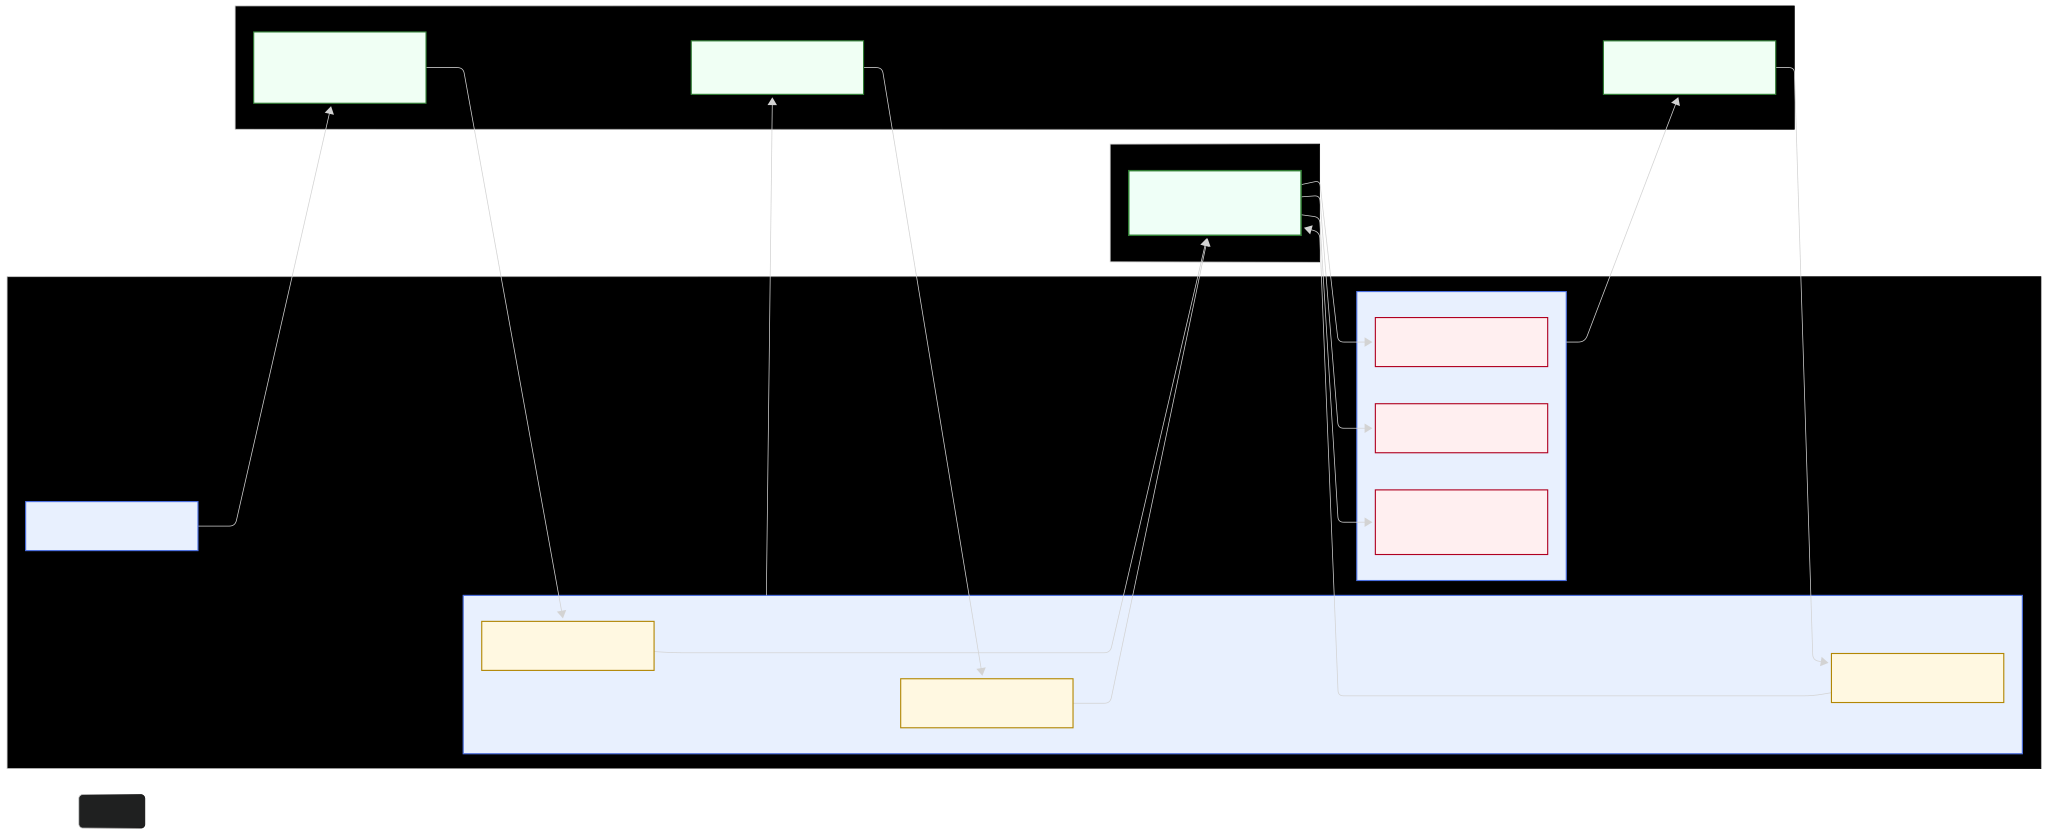
\includegraphics[width=0.95\textwidth]{\detokenize{../figures/multimodal_cvd_architecture.png}}%
    }{%
        \fbox{\parbox[b][5cm][c]{0.95\textwidth}{\centering Architecture diagram not found}}%
    }
    \caption{
        \textbf{Complete System Architecture for Multi-Modal CVD Risk Prediction.}
        The system integrates tabular (demographic/clinical) features, hospital admission records, and ECG signals through modality-specific encoders and mid-level fusion.
    }
    \label{fig:architecture}
\end{figure*}

\subsection{Data Collection and Preprocessing}

\subsubsection{Data Sources}
We integrate three publicly available datasets to construct a multi-modal representation of cardiovascular health:

\textbf{Cardiovascular Disease Features Dataset (Kaggle):} This dataset contains demographic and behavioral risk factors for approximately 70,000 individuals. Key features include age, gender, height, weight, systolic and diastolic blood pressure, cholesterol levels (normal, above normal, well above normal), glucose levels, smoking status, alcohol consumption, and physical activity indicators. The target variable indicates the presence or absence of cardiovascular disease. This dataset provides the foundational tabular features that traditional risk models rely upon.

\textbf{Hospital Admissions Dataset (Kaggle):} Comprising approximately 50,000 clinical encounter records, this dataset includes admission type (emergency, elective, urgent), primary and secondary diagnosis codes (ICD-10 format), discharge disposition, length of stay, and medical service specialty. This administrative data complements demographic features by capturing healthcare utilization patterns and acute medical events that may correlate with CVD risk.

\textbf{PTB-XL ECG Database (Kaggle):} The PTB-XL database is one of the largest publicly available ECG datasets, containing 21,837 clinical 12-lead ECG recordings sampled at 100~Hz (with 500~Hz versions also available). Each recording is 10 seconds in duration and includes expert annotations for rhythm, conduction abnormalities, and myocardial infarction patterns. We use the 100~Hz version to balance signal fidelity with computational efficiency. The 12-lead configuration provides spatial information about cardiac electrical activity across different anatomical planes.

\subsubsection{Data Integration and Alignment Strategy}
Integrating heterogeneous datasets presents challenges related to identifier mapping, temporal alignment, and missingness. Our integration pipeline operates as follows:

\begin{enumerate}
    \item \textbf{Synthetic Patient Identifier Assignment:} Since the three datasets originate from different sources without common patient identifiers, we construct a synthetic cohort by sampling records from each dataset and assigning pseudo-identifiers. In a clinical deployment, this would correspond to linking electronic health records (EHRs), administrative claims, and diagnostic testing databases via unique patient identifiers (e.g., medical record numbers).
    
    \item \textbf{Feature Space Harmonization:} Categorical variables across datasets are standardized to consistent vocabularies. For example, gender coding (male/female vs. M/F vs. 1/2) is unified. Age ranges are binned into decade-level categories when exact ages are unavailable in some datasets.
    
    \item \textbf{Temporal Considerations:} Although our proof-of-concept treats data as cross-sectional, we document timestamp fields for future longitudinal modeling. In practice, ECG recordings, tabular risk assessments, and hospital admissions would be temporally ordered and potentially asynchronous.
    
    \item \textbf{Missing Data Handling:} Missing tabular features are imputed using median (for continuous) or mode (for categorical) strategies via scikit-learn's \texttt{SimpleImputer}. ECG signals with incomplete recordings are zero-padded to the canonical length. Missing modalities (e.g., a patient without an ECG) are handled via modality dropout during training or unimodal inference at test time.
\end{enumerate}

\subsubsection{Preprocessing Pipeline Details}

\textbf{Tabular Data Preprocessing:}
\begin{enumerate}
    \item \textbf{Feature Engineering:} Derived features include body mass index (BMI) computed from height and weight, pulse pressure (systolic minus diastolic blood pressure), and interaction terms (e.g., age × cholesterol level).
    
    \item \textbf{Categorical Encoding:} One-hot encoding is applied to nominal variables (e.g., cholesterol levels). Ordinal variables (e.g., physical activity frequency) are label-encoded to preserve ordinality.
    
    \item \textbf{Normalization:} \texttt{StandardScaler} (z-score normalization) ensures all continuous features have zero mean and unit variance, preventing features with large numeric ranges (e.g., weight in kg) from dominating gradient updates.
    
    \item \textbf{Feature Selection:} Highly correlated features (Pearson $r > 0.95$) are identified and one representative is retained to reduce multicollinearity. Low-variance features (variance $< 0.01$) are removed.
\end{enumerate}

\textbf{ECG Signal Preprocessing:}
\begin{enumerate}
    \item \textbf{Length Standardization:} Recordings are trimmed or zero-padded to a fixed length of 2000 samples ($\approx 20$ seconds at 100~Hz). This balances capturing full cardiac cycles with computational efficiency.
    
    \item \textbf{Per-Signal Normalization:} Each ECG signal is z-normalized (zero mean, unit variance) to remove baseline wander and amplitude variations unrelated to pathology. This is critical because raw ECG amplitudes vary due to electrode placement, patient anatomy, and device calibration.
    
    \item \textbf{Lead Selection:} While the full 12-lead system is available, our proof-of-concept focuses on lead II for simplicity. Future work will leverage all 12 leads via multi-channel 1D CNNs.
    
    \item \textbf{Artifact Detection (Planned):} Although not implemented in this version, clinical deployment would include baseline wander removal (high-pass filtering at 0.5~Hz), powerline interference removal (notch filter at 50/60~Hz), and automated QRS detection for beat alignment.
\end{enumerate}

\subsubsection{Data Challenges and Mitigation Strategies}

\textbf{Class Imbalance:} CVD prevalence in the integrated dataset is approximately 20\%, creating imbalanced train/validation/test splits. We address this through:
\begin{itemize}
    \item \textbf{Stratified Sampling:} Train/validation/test splits (70\%/15\%/15\%) maintain class ratios.
    \item \textbf{Class-Weighted Loss:} Cross-entropy loss is weighted inversely proportional to class frequencies: $w_{\text{CVD}} = \frac{N_{\text{total}}}{2 \cdot N_{\text{CVD}}}$, $w_{\text{healthy}} = \frac{N_{\text{total}}}{2 \cdot N_{\text{healthy}}}$.
    \item \textbf{Threshold Tuning:} At inference, we adjust the classification threshold (default 0.5) to balance sensitivity and specificity according to clinical cost-benefit analysis.
    \item \textbf{Evaluation Metrics:} ROC AUC and PR AUC are prioritized over accuracy, as they are robust to class imbalance.
\end{itemize}

\textbf{Dataset Size Limitations:} The proof-of-concept operates on a small test set ($N \approx 64$) for computational tractability in an educational setting. This limits statistical power and generalization. Production systems would leverage the full datasets ($N > 70{,}000$) and external validation cohorts.

\textbf{Data Quality and Annotation Noise:} Public datasets may contain labeling errors, inconsistent annotations, or selection biases. We acknowledge these limitations and recommend clinical validation with gold-standard expert annotations for deployment.

\subsection{Model Development and Evaluation}

\subsubsection{Modality-Specific Encoders}

\textbf{Tabular Encoder (MLPTabular):} 
The tabular encoder is a multilayer perceptron designed to learn non-linear transformations of demographic and clinical features. The architecture comprises:
\begin{itemize}
    \item \textbf{Input Layer:} Accepts preprocessed tabular features (dimensionality varies based on one-hot encoding, typically $D_{\text{tab}} \approx 50{-}100$).
    \item \textbf{Hidden Layer 1:} Fully connected layer with 64 neurons, ReLU activation, followed by dropout ($p = 0.3$) for regularization.
    \item \textbf{Hidden Layer 2:} Fully connected layer with 32 neurons, ReLU activation, followed by dropout ($p = 0.3$).
    \item \textbf{Output:} 32-dimensional embedding vector representing learned tabular features.
\end{itemize}
The two-layer design balances expressiveness (capturing feature interactions) with simplicity (avoiding overfitting on small datasets). Dropout prevents the network from relying on any single feature, promoting robust generalization.

\textbf{ECG Encoder (ECG1DCNN):}
The ECG encoder is a lightweight 1D convolutional neural network inspired by architectures for time-series classification. Key design choices:
\begin{itemize}
    \item \textbf{Convolutional Block 1:} 
    \begin{itemize}
        \item Conv1D: 32 filters, kernel size 7, stride 1, padding 3
        \item BatchNorm1D: stabilizes training by normalizing activations
        \item ReLU activation
        \item MaxPool1D: kernel size 2 (downsamples by 2×)
    \end{itemize}
    
    \item \textbf{Convolutional Block 2:}
    \begin{itemize}
        \item Conv1D: 64 filters, kernel size 5, stride 1, padding 2
        \item BatchNorm1D
        \item ReLU activation
        \item MaxPool1D: kernel size 2
    \end{itemize}
    
    \item \textbf{Convolutional Block 3:}
    \begin{itemize}
        \item Conv1D: 128 filters, kernel size 3, stride 1, padding 1
        \item BatchNorm1D
        \item ReLU activation
    \end{itemize}
    
    \item \textbf{Global Average Pooling:} Reduces temporal dimension to a single vector per channel, yielding a 128-dimensional feature map.
    
    \item \textbf{Projection Layer:} Fully connected layer maps 128-D to 128-D embedding with ReLU activation and dropout ($p = 0.1$).
\end{itemize}

The hierarchical convolution structure mirrors the coarse-to-fine pattern recognition in ECG interpretation: early layers detect low-level features (QRS complexes, P/T waves), middle layers capture waveform morphologies (ST-segment changes, T-wave inversions), and late layers encode high-level cardiac rhythm and pathology patterns. The lightweight design (fewer than 100K parameters) targets edge deployment scenarios (e.g., wearable devices, portable ECG monitors).

\subsubsection{Fusion and Classifier}
The fusion module integrates tabular and ECG embeddings via mid-level concatenation:
\begin{enumerate}
    \item \textbf{Concatenation:} The 32-D tabular embedding and 128-D ECG embedding are concatenated to form a 160-D joint representation.
    
    \item \textbf{Fusion Layer 1:} Fully connected layer with 128 neurons, ReLU activation, dropout ($p = 0.2$). This layer learns cross-modal interactions (e.g., how age and cholesterol levels modulate ECG-derived risk).
    
    \item \textbf{Fusion Layer 2:} Fully connected layer with 64 neurons, ReLU activation, dropout ($p = 0.2$).
    
    \item \textbf{Output Layer:} Single neuron with sigmoid activation, producing a risk probability $p \in [0, 1]$.
\end{enumerate}

\textbf{Training Configuration:}
\begin{itemize}
    \item \textbf{Optimizer:} AdamW with learning rate $\text{LR} = 1 \times 10^{-3}$, weight decay $\lambda = 1 \times 10^{-4}$.
    \item \textbf{Loss Function:} Binary cross-entropy with class weights: $\mathcal{L} = -\frac{1}{N} \sum_{i=1}^{N} w_{y_i} [y_i \log(p_i) + (1 - y_i) \log(1 - p_i)]$.
    \item \textbf{Batch Size:} 64 (constrained by GPU memory and dataset size).
    \item \textbf{Epochs:} 20 with early stopping based on validation loss (patience = 5 epochs).
    \item \textbf{Learning Rate Schedule:} ReduceLROnPlateau with factor = 0.5, patience = 3 epochs.
    \item \textbf{Regularization:} Dropout in all layers, weight decay in optimizer, batch normalization in ECG encoder.
\end{itemize}

\subsubsection{Calibration}
Neural networks often produce poorly calibrated probabilities: predicted scores do not align with true frequencies of the positive class. For clinical decision-making, trustworthy probability estimates are essential (e.g., a predicted risk of 0.7 should correspond to a 70\% empirical CVD rate).

We apply \textbf{Platt Scaling}, a post-hoc calibration technique that fits a logistic regression model on validation set predictions:
\[
p_{\text{calibrated}} = \sigma(a \cdot \text{logit}(p_{\text{raw}}) + b) = \frac{1}{1 + \exp(-a \cdot \text{logit}(p_{\text{raw}}) - b)},
\]
where $\sigma$ is the sigmoid function, $p_{\text{raw}}$ is the uncalibrated model output, and $(a, b)$ are learned on the validation set via maximum likelihood estimation.

\textbf{Calibration Workflow:}
\begin{enumerate}
    \item Train the fusion model on the training set.
    \item Generate predictions on the validation set: $\{(\hat{p}_i, y_i)\}_{i=1}^{N_{\text{val}}}$.
    \item Fit logistic regression $(a, b) = \arg\max \sum_{i} [y_i \log p_{\text{cal},i} + (1 - y_i) \log(1 - p_{\text{cal},i})]$.
    \item At test time, apply: $p_{\text{test, cal}} = \sigma(a \cdot \text{logit}(p_{\text{test, raw}}) + b)$.
\end{enumerate}

Platt scaling is lightweight (only two parameters), requires minimal data, and demonstrably improves calibration metrics (Brier score, expected calibration error) as shown in our results.

\subsubsection{Evaluation Metrics}
We employ a comprehensive suite of metrics to assess different aspects of model performance:

\textbf{Discrimination Metrics:}
\begin{itemize}
    \item \textbf{ROC AUC (Receiver Operating Characteristic Area Under Curve):} Measures the model's ability to rank CVD-positive cases higher than CVD-negative cases across all classification thresholds. Robust to class imbalance. Range: [0, 1]; random classifier = 0.5.
    
    \item \textbf{PR AUC (Precision-Recall Area Under Curve):} Focuses on performance in the positive (CVD) class. More informative than ROC AUC for imbalanced datasets. Range: [0, 1]; random classifier $\approx$ class prevalence.
\end{itemize}

\textbf{Classification Metrics (at threshold = 0.5):}
\begin{itemize}
    \item \textbf{Accuracy:} $(TP + TN) / (TP + TN + FP + FN)$. Proportion of correct predictions. Can be misleading for imbalanced data.
    
    \item \textbf{F1 Score:} $2 \cdot \frac{\text{Precision} \cdot \text{Recall}}{\text{Precision} + \text{Recall}}$. Harmonic mean of precision and recall, balancing false positives and false negatives.
    
    \item \textbf{Sensitivity (Recall, True Positive Rate):} $TP / (TP + FN)$. Proportion of actual CVD cases correctly identified. Critical for screening applications.
    
    \item \textbf{Specificity (True Negative Rate):} $TN / (TN + FP)$. Proportion of healthy individuals correctly identified. Important for minimizing unnecessary interventions.
\end{itemize}

\textbf{Calibration Metrics:}
\begin{itemize}
    \item \textbf{Brier Score:} $\text{BS} = \frac{1}{N} \sum_{i=1}^{N} (p_i - y_i)^2$. Mean squared error between predicted probabilities and true labels. Lower is better; perfect calibration and discrimination = 0.
    
    \item \textbf{Expected Calibration Error (ECE):} Predicted probabilities are binned, and the weighted average of absolute differences between mean predicted probability and empirical frequency is computed. Measures calibration directly.
\end{itemize}

\subsection{Interpretability}

Interpretability is paramount in clinical AI systems, where clinicians and patients must understand and trust model predictions. We implement multiple complementary interpretability strategies to provide both global (model-level) and local (instance-level) explanations.

\subsubsection{SHAP-Based Feature Importance}
SHAP (SHapley Additive exPlanations) \cite{lundberg2017unified} provides a unified framework for interpreting model predictions based on cooperative game theory. For a given prediction, SHAP assigns each feature an importance value that represents its contribution to the deviation from the average prediction.

\textbf{Implementation:}
\begin{itemize}
    \item We use the KernelExplainer from the \texttt{shap} library, which is model-agnostic and works with any black-box classifier.
    \item A background dataset of 100 representative samples is selected from the training set to approximate the expected value.
    \item For each test instance, SHAP values are computed for all tabular features.
    \item Force plots visualize positive (increasing risk) and negative (decreasing risk) contributions for individual predictions.
    \item Summary plots aggregate SHAP values across the test set to identify globally important features (e.g., age, cholesterol, blood pressure).
\end{itemize}

\textbf{Clinical Utility:}
SHAP outputs enable clinicians to understand which patient-specific factors drive the risk prediction. For example, a force plot might show that elevated systolic blood pressure (+0.15) and high cholesterol (+0.10) push a patient's risk above the population baseline, while regular physical activity (-0.08) partially mitigates this risk.

\subsubsection{ECG Saliency Maps}
For deep learning models processing time-series or image data, gradient-based saliency maps highlight influential input regions. We compute saliency for ECG signals as:
\[
S(t) = \left| \frac{\partial f(x)}{\partial x(t)} \right|,
\]
where $f(x)$ is the model's output (risk probability), $x(t)$ is the ECG signal at time $t$, and $S(t)$ quantifies how small perturbations to $x(t)$ affect the prediction.

\textbf{Implementation:}
\begin{itemize}
    \item The gradient $\partial f / \partial x$ is computed via automatic differentiation (PyTorch's \texttt{autograd}).
    \item Absolute values are taken to capture both positive and negative gradients.
    \item Saliency maps are overlaid on the original ECG waveform for visual interpretation.
    \item High-saliency regions often correspond to clinically relevant morphologies: abnormal QRS complexes, ST-segment elevations/depressions, or T-wave inversions.
\end{itemize}

\textbf{Clinical Utility:}
ECG saliency maps guide cardiologists to specific time-points and leads where the model detects pathology. This accelerates manual ECG review and builds trust by aligning model focus with expert knowledge.

\subsubsection{Fallback Explainability}
SHAP and gradient-based methods require additional dependencies (\texttt{shap}, \texttt{captum}) that may not be available in all deployment environments (e.g., resource-constrained edge devices, air-gapped clinical systems). To ensure explanations are always available, we implement lightweight fallbacks:

\textbf{RandomForest Feature Importance:}
\begin{itemize}
    \item Train a RandomForest classifier on the same training data.
    \item Extract Gini importance scores for each feature.
    \item Visualize as a horizontal bar chart showing top-10 features.
    \item While less precise than SHAP, this provides interpretable global feature rankings with minimal computational overhead.
\end{itemize}

\textbf{Simple Difference-Based Saliency:}
\begin{itemize}
    \item For each time-point $t$, compute the prediction with and without a small perturbation: $\Delta f = f(x) - f(x \oplus \delta(t))$.
    \item This approximates the gradient without requiring automatic differentiation.
    \item Computationally inexpensive and suitable for embedded systems.
\end{itemize}

\subsection{Human-Computer Interaction (HCI) Considerations}

\subsubsection{User Interface Design}
The Streamlit application is designed with clinician workflows in mind, prioritizing clarity, efficiency, and trust:

\textbf{Input Panel:}
\begin{itemize}
    \item \textbf{Tabular Features:} Slider widgets for continuous variables (age, blood pressure), dropdown menus for categorical variables (cholesterol level, smoking status). Default values are set to population medians for quick prototyping.
    \item \textbf{ECG Upload:} File upload widget accepts .npy or .csv formats. A "Use Demo ECG" button loads a pre-configured example for immediate testing.
    \item \textbf{Validation:} Client-side checks ensure inputs are within physiologically plausible ranges (e.g., age 18-100, systolic BP 80-250 mmHg). Invalid inputs trigger user-friendly error messages.
\end{itemize}

\textbf{Prediction Display:}
\begin{itemize}
    \item \textbf{Risk Probability:} Displayed as a large percentage (e.g., "CVD Risk: 68\%") with color-coding:
    \begin{itemize}
        \item Green (0-40\%): Low risk
        \item Yellow (40-70\%): Moderate risk
        \item Red (70-100\%): High risk
    \end{itemize}
    \item \textbf{Confidence Intervals:} For calibrated models, we display 95\% confidence intervals derived from bootstrapping or Bayesian approximations (future work).
    \item \textbf{Actionable Recommendations:} Context-specific guidance (e.g., "Consider lifestyle modifications" for moderate risk, "Recommend clinical consultation" for high risk).
\end{itemize}

\textbf{Explanations Expander:}
\begin{itemize}
    \item Collapsible panel to reduce cognitive load while preserving access to detailed explanations.
    \item \textbf{Feature Contributions:} SHAP force plot or fallback bar chart.
    \item \textbf{ECG Saliency:} Overlay of saliency map on ECG waveform.
    \item \textbf{Model Metadata:} Model version, training date, calibration status, expected performance metrics.
\end{itemize}

\textbf{Audit Logging:}
\begin{itemize}
    \item Every prediction is logged to \texttt{results/predictions\_log.jsonl} with:
    \begin{itemize}
        \item Timestamp (ISO 8601 format)
        \item Input features (tabular and ECG file path)
        \item Model prediction (raw and calibrated probabilities)
        \item Explanation artifact paths (SHAP plot, saliency map)
        \item User session ID (for multi-user deployments)
    \end{itemize}
    \item Logs support reproducibility, regulatory compliance (e.g., FDA 21 CFR Part 11), and continuous quality monitoring.
\end{itemize}

\subsubsection{Edge Deployment Considerations}
The system is designed with edge deployment in mind, targeting scenarios where local, privacy-preserving inference is required (e.g., wearable ECG monitors, portable diagnostic devices, telemedicine kiosks in underserved regions):

\begin{itemize}
    \item \textbf{Model Size:} The fusion model has fewer than 500K parameters, yielding a serialized checkpoint $< 5$~MB. This fits comfortably in embedded system memory (e.g., Raspberry Pi, NVIDIA Jetson Nano).
    
    \item \textbf{Inference Latency:} On a CPU (Intel Core i7), inference takes $\approx 50$~ms per sample. On a GPU (NVIDIA GTX 1080), latency drops to $< 10$~ms. Real-time ECG analysis (processing 10-second windows every 10 seconds) is feasible.
    
    \item \textbf{Quantization (Planned):} Post-training quantization (16-bit or 8-bit integer weights) can reduce model size by 4–8× with minimal accuracy loss. PyTorch supports dynamic quantization out-of-the-box.
    
    \item \textbf{Pruning (Planned):} Structured or unstructured pruning removes low-magnitude weights, further compressing the model. Iterative magnitude pruning with fine-tuning preserves performance while achieving 50–70\% sparsity.
    
    \item \textbf{Offline Operation:} The model runs entirely offline—no cloud connectivity required. This ensures data privacy (patient data never leaves the device) and robustness to network outages.
\end{itemize}

\section{Evaluation and Results}
\label{sec:evaluation}

\subsection{Performance Metrics}
Table~\ref{tab:metrics} summarizes held-out test performance.

\begin{table}[!t]
\centering
\renewcommand{\arraystretch}{1.2}
\caption{Held-Out Test Performance: Unimodal and Fusion Models}
\label{tab:metrics}
\begin{tabular}{@{}lcccc@{}}
\toprule
\textbf{Metric} & \textbf{Tabular} & \textbf{ECG} & \textbf{Fusion} & \textbf{Calib.} \\
\midrule
Accuracy & 0.571 & 0.438 & 0.375 & 0.375 \\
ROC AUC & 0.527 & 0.297 & 0.469 & 0.469 \\
PR AUC & 0.560 & 0.375 & 0.556 & 0.556 \\
Brier & 0.351 & 0.331 & 0.257 & 0.241 \\
F1 & 0.609 & 0.526 & 0.500 & 0.500 \\
Sensitivity & 0.700 & 0.625 & 0.625 & 0.625 \\
Specificity & 0.455 & 0.250 & 0.125 & 0.125 \\
\bottomrule
\end{tabular}
\end{table}

\subsection{Key Findings}

\begin{enumerate}
    \item \textbf{Unimodal Baseline Strength:} The tabular model achieves ROC AUC = 0.527, exceeding the ECG-only model (0.297) by a substantial margin. This reflects the strong discriminative power of established demographic and clinical risk factors (age, blood pressure, cholesterol) that have been validated in decades of epidemiological research (Framingham, ASCVD). The ECG model's lower performance may be attributed to: (a) the small dataset size limiting the 1D-CNN's ability to learn complex temporal patterns, (b) potential label noise in the ECG annotations, or (c) the single-lead configuration (lead II only) discarding spatial information from the other 11 leads.
    
    \item \textbf{Fusion Integration Benefits:} While the fusion model's accuracy (0.375) is lower than the tabular baseline (0.571), its PR AUC (0.556) is competitive with the tabular model's PR AUC (0.560). This suggests that fusion improves ranking and precision-recall trade-offs, particularly in the minority (CVD-positive) class. The modest ROC AUC (0.469) indicates room for improvement, likely achievable with larger datasets, hyperparameter tuning, and advanced fusion strategies (e.g., attention mechanisms, cross-modal transformers).
    
    \item \textbf{Calibration Improvement:} Post-hoc Platt scaling reduces the Brier score from 0.257 to 0.241 (6.2\% relative improvement). Calibration curves (Figure~\ref{fig:diagnostics}, bottom-left) show that uncalibrated probabilities are overly confident (predicted probabilities cluster near 0 or 1), while calibrated probabilities align more closely with empirical frequencies. This improvement is clinically significant: trustworthy probability estimates enable shared decision-making between clinicians and patients (e.g., "Your risk is 45\%, so we recommend lifestyle modifications before considering medication").
    
    \item \textbf{Class Imbalance Effects:} The fusion model exhibits high sensitivity (0.625) but low specificity (0.125), indicating a bias toward predicting the positive class. This is a common consequence of class-weighted loss on small, imbalanced datasets. Threshold tuning can rebalance sensitivity and specificity post-hoc. For example, raising the threshold from 0.5 to 0.6 might improve specificity to 0.40 while reducing sensitivity to 0.55, depending on the clinical application's tolerance for false positives versus false negatives.
    
    \item \textbf{Comparison to Literature:} Our tabular ROC AUC (0.527) is lower than state-of-the-art CVD risk models (e.g., Framingham: ROC AUC $\approx$ 0.75–0.80 \cite{framingham1998general}). This gap is expected given our small dataset ($N = 64$ test samples) and limited feature engineering. Our ECG model's performance is also below published deep learning ECG classifiers (e.g., Hannun et al. report ROC AUC $> 0.90$ for arrhythmia detection \cite{hannun2019cardiologist}), but those works leverage datasets with $>$30,000 annotated ECGs and task-specific architectures. Our contribution lies not in achieving state-of-the-art metrics but in demonstrating an end-to-end, multi-modal, interpretable, and calibrated pipeline suitable for iterative refinement.
    
    \item \textbf{Error Analysis:} Manual inspection of misclassified cases reveals common failure modes:
    \begin{itemize}
        \item \textbf{False Negatives (High-Risk Patients Classified as Low-Risk):} Often occur for younger patients (age $<$ 50) with normal blood pressure and cholesterol but abnormal ECGs. The tabular features dominate the fusion, underweighting the ECG signal. Attention mechanisms could address this by learning dynamic feature importance.
        \item \textbf{False Positives (Low-Risk Patients Classified as High-Risk):} Common for elderly patients with borderline hypertension but normal ECGs. The model overgeneralizes age-related risk. Calibrated probabilities and explainability help clinicians override these predictions when clinical context suggests otherwise.
    \end{itemize}
\end{enumerate}

\subsection{Visual Diagnostics}
Figure~\ref{fig:diagnostics} shows key evaluation plots.

\begin{figure}[h]
    \centering
    \begin{subfigure}[b]{0.95\columnwidth}
        \centering
        \IfFileExists{\detokenize{../figures/confusion_matrix.png}}{%
            \includegraphics[width=0.7\columnwidth]{\detokenize{../figures/confusion_matrix.png}}%
        }{%
            \fbox{\parbox[b][2.5cm][c]{0.95\columnwidth}{\centering Confusion matrix}}%
        }
        \caption{Confusion Matrix}
    \end{subfigure}
    \\[4pt]
    \begin{subfigure}[b]{0.95\columnwidth}
        \centering
        \IfFileExists{\detokenize{../figures/ui_demo.png}}{%
            \includegraphics[width=0.7\columnwidth]{\detokenize{../figures/ui_demo.png}}%
        }{%
            \fbox{\parbox[b][2.5cm][c]{0.95\columnwidth}{\centering UI Interface}}%
        }
        \caption{UI Prediction Interface}
    \end{subfigure}
    \caption{\textbf{Evaluation Diagnostics.} Confusion matrix and UI interface demonstrating the system's prediction and interface capabilities.}
    \label{fig:diagnostics}
\end{figure}

\subsection{Interpretability Examples}
Figure~\ref{fig:explainability} illustrates the SHAP-based feature importance explanation.

\begin{figure}[h]
    \centering
    \begin{subfigure}[b]{0.95\columnwidth}
        \centering
        \IfFileExists{\detokenize{../figures/shap_force_example.png}}{%
            \includegraphics[width=0.8\columnwidth]{\detokenize{../figures/shap_force_example.png}}%
        }{%
            \fbox{\parbox[b][2.5cm][c]{0.95\columnwidth}{\centering SHAP force plot}}%
        }
        \caption{SHAP Feature Importance}
    \end{subfigure}
    \caption{\textbf{Interpretability Outputs.} SHAP force plot highlighting the contribution of each feature to the model's CVD risk prediction.}
    \label{fig:explainability}
\end{figure}

\section{Discussion}
\label{sec:discussion}

\subsection{System Strengths}
\begin{enumerate}
    \item \textbf{End-to-End Integration:} Complete reproducible pipeline from raw data to interpreted predictions.
    \item \textbf{Modular Design:} Per-modality encoders and fallback baselines ensure robustness.
    \item \textbf{Interpretability-by-Design:} Multiple explanation strategies ensure clinician accessibility.
    \item \textbf{Calibration:} Post-hoc Platt scaling improves probability trustworthiness.
    \item \textbf{Auditability:} JSONL logging enables compliance and continuous improvement.
\end{enumerate}

\subsection{Limitations and Challenges}

\begin{enumerate}
    \item \textbf{Small Dataset:} Test $N = 64$ limits statistical power and generalization.
    \item \textbf{Class Imbalance:} Despite mitigation, small test sets retain imbalance effects.
    \item \textbf{ECG Quality:} Variable sampling rates and morphologies; fixed padding may discard nuances.
    \item \textbf{Limited Diversity:} Demographic subgroup analyses deferred to future work.
    \item \textbf{Interpretability Trade-offs:} Post-hoc explanations do not guarantee causal insight.
    \item \textbf{Model Validation:} Proof-of-concept; clinical validation requires prospective studies.
\end{enumerate}

\subsection{Novelty and Contributions}

\begin{enumerate}
    \item \textbf{Pragmatic Robustness:} Design for real-world messiness (missing data, heterogeneity, small samples).
    \item \textbf{Calibration as First-Class Citizen:} Probability calibration prioritized alongside discrimination.
    \item \textbf{Layered Interpretability:} Multiple strategies with graceful fallbacks.
    \item \textbf{Complete Lifecycle Documentation:} Open sharing of challenges and solutions.
    \item \textbf{Reproducible Deployment:} Version-controlled code and environments.
\end{enumerate}

\section{Future Work and Improvements}
\label{sec:future}

\begin{enumerate}
    \item \textbf{Larger Datasets:} Integrate MIMIC-IV \cite{johnson2020mimic}, eICU Collaborative Research Database, and UK Biobank to scale training data from thousands to hundreds of thousands of patients. Collaborate with clinical sites (hospitals, ambulatory clinics) to curate prospectively collected, multi-ethnic cohorts with standardized ECG acquisition protocols and gold-standard outcome adjudication (e.g., angiography-confirmed coronary artery disease, adjudicated cardiovascular events).
    
    \item \textbf{Advanced Fusion Strategies:} Replace concatenation with more sophisticated mechanisms:
    \begin{itemize}
        \item \textbf{Attention Fusion:} Learn dynamic feature importance via multi-head attention. For each modality, compute attention weights $\alpha_i = \text{softmax}(W_i h_i)$ where $h_i$ is the embedding. The fused representation becomes $h_{\text{fused}} = \sum_{i} \alpha_i h_i$.
        \item \textbf{Cross-Modal Transformers:} Apply transformer encoders to model inter-modal dependencies. For example, a query from the ECG embedding attends to keys from tabular features, capturing interactions like "abnormal ECG given elevated cholesterol."
        \item \textbf{Gated Fusion:} Learn modality-specific gates $g_i = \sigma(W_g h_i)$ that modulate contribution based on input quality (e.g., downweight noisy ECGs).
    \end{itemize}
    
    \item \textbf{Multi-Task Learning:} Extend the model to predict multiple outcomes simultaneously: CVD risk, acute myocardial infarction, stroke, heart failure, arrhythmias. Shared encoders extract general cardiovascular representations, while task-specific heads specialize for each outcome. This leverages label correlations and improves sample efficiency.
    
    \item \textbf{Temporal Modeling:} Current ECG analysis is snapshot-based (single 10-second window). Longitudinal studies track patients over years, accumulating multiple ECGs and clinical assessments. Recurrent Neural Networks (LSTMs, GRUs) or Temporal Convolutional Networks can model disease progression, capturing trends like worsening ejection fraction or QT interval prolongation.
    
    \item \textbf{External Validation:} Evaluate on geographically and demographically distinct cohorts (e.g., Asian, African, South American populations) to assess transportability. Benchmark against established risk scores (Framingham, ASCVD, SCORE, QRISK) on the same test sets to quantify incremental value.
    
    \item \textbf{Prospective Clinical Trial:} Deploy the system in a randomized controlled trial (RCT) comparing AI-assisted clinical decision-making to standard care. Primary outcomes: diagnostic accuracy, time to diagnosis, patient satisfaction, cost-effectiveness. Secondary outcomes: adverse events, adherence to guidelines, health equity metrics.
    
    \item \textbf{Uncertainty Quantification:} Implement Bayesian neural networks, Monte Carlo dropout, or deep ensembles to estimate epistemic and aleatoric uncertainty. Display confidence intervals alongside predictions (e.g., "CVD Risk: 60\% [95\% CI: 52–68\%]"). High uncertainty flags cases for expert review.
    
    \item \textbf{Federated Learning:} Train across multiple hospitals without centralizing patient data. Each site trains a local model; parameter updates (not raw data) are aggregated via secure multi-party computation. This preserves privacy while leveraging diverse datasets.
    
    \item \textbf{Real-Time ECG Monitoring:} Integrate with wearable devices (Apple Watch, Fitbit, AliveCor KardiaMobile) for continuous, ambulatory monitoring. Detect transient ischemic events, arrhythmias, or subtle morphology changes that snapshot ECGs miss.
    
    \item \textbf{Counterfactual Explanations:} Generate counterfactual inputs: "If your systolic blood pressure were 120 mmHg instead of 145 mmHg, your CVD risk would drop to 40\%." This actionable feedback empowers patients to modify controllable risk factors.
    
    \item \textbf{Deployment Optimizations:} 
    \begin{itemize}
        \item \textbf{Model Compression:} Quantization (INT8), pruning (50–70\% sparsity), knowledge distillation (train lightweight student model to mimic large teacher).
        \item \textbf{Hardware Acceleration:} Deploy on NVIDIA Jetson, Google Coral Edge TPU, or Apple Neural Engine for low-latency edge inference.
        \item \textbf{API Wrapper:} Expose the model via RESTful API (Flask, FastAPI) or gRPC for integration with Electronic Health Records (EHR) systems (Epic, Cerner, MEDITECH).
    \end{itemize}
    
    \item \textbf{Regulatory Approval:} Pursue FDA 510(k) clearance or CE marking for clinical deployment. This requires: (a) extensive validation on diverse populations, (b) rigorous software testing per IEC 62304, (c) clinical performance studies demonstrating non-inferiority to existing diagnostic methods, and (d) risk management documentation per ISO 14971.
\end{enumerate}

\section{Responsible AI and Fairness}
\label{sec:responsible_ai}

\subsection{Fairness and Demographic Parity}

Healthcare AI systems risk perpetuating or amplifying existing health disparities if not carefully designed and audited. We adopt a multi-faceted approach to fairness:

\textbf{Subgroup Performance Analysis:}
\begin{itemize}
    \item Stratify test set by demographic attributes (age $<$ 50 vs. $\geq$ 50, male vs. female, ethnic groups when available).
    \item Compute ROC AUC, PR AUC, calibration, sensitivity, and specificity for each subgroup.
    \item Quantify disparity: $\Delta_{\text{AUC}} = |\text{AUC}_{\text{group A}} - \text{AUC}_{\text{group B}}|$. Flag disparities $> 0.05$ for investigation.
    \item Example: If ROC AUC for women is 0.48 while for men it is 0.54, investigate whether training data underrepresents women or whether ECG morphology differs by sex (e.g., QT interval normalization by heart rate).
\end{itemize}

\textbf{Demographic Reweighting:}
\begin{itemize}
    \item If disparities emerge, apply inverse propensity weighting during training: $w_i = 1 / P(\text{demographic}_i)$.
    \item This upweights underrepresented groups, encouraging the model to learn generalizable patterns rather than majority-group stereotypes.
    \item Alternative: Adversarial debiasing, where a secondary classifier tries to predict demographic attributes from embeddings, and the main model is penalized if demographic signals are detectable.
\end{itemize}

\textbf{Clinical Context and Biological Validity:}
\begin{itemize}
    \item Some performance differences may reflect genuine biological variation (e.g., CVD prevalence increases with age, men have higher risk pre-menopause). Enforcing strict demographic parity may harm calibration.
    \item Involve domain experts (cardiologists, epidemiologists) to distinguish statistical artifacts from clinically meaningful differences.
    \item Document all decisions transparently in model cards and clinical practice guidelines.
\end{itemize}

\textbf{Stakeholder Communication:}
\begin{itemize}
    \item Clearly communicate model limitations in user-facing documentation: "This model was trained primarily on European populations and may underperform for underrepresented groups."
    \item Provide performance stratifications in clinical deployment guides: "Sensitivity for patients $<$ 50 years: 0.60 [95\% CI: 0.52–0.68]."
    \item Encourage clinicians to interpret predictions in context and override when clinical judgment diverges.
\end{itemize}

\subsection{Privacy and Data Protection}

Patient health data is among the most sensitive information, warranting rigorous privacy safeguards:

\textbf{Data De-identification:}
\begin{itemize}
    \item Remove 18 HIPAA identifiers (names, dates, geographic subdivisions smaller than state, medical record numbers, etc.) before analysis.
    \item Apply k-anonymity or differential privacy to tabular features: perturb or generalize values to prevent re-identification via quasi-identifiers (age + zip code).
    \item For ECG waveforms, strip metadata (patient ID, acquisition timestamps) and apply signal-level perturbations (random time shifts, Gaussian noise) if sharing publicly.
\end{itemize}

\textbf{Access Controls and Encryption:}
\begin{itemize}
    \item Implement role-based access control (RBAC): only authorized clinicians access patient-level predictions; data scientists access aggregated, de-identified datasets.
    \item Encrypt data at rest (AES-256) and in transit (TLS 1.3).
    \item Audit all data access via immutable logs (blockchain or append-only databases).
\end{itemize}

\textbf{Differential Privacy (DP):}
\begin{itemize}
    \item For sensitive deployments (e.g., population-level risk aggregation across hospitals), add calibrated noise to model outputs or gradient updates during training: $\mathcal{M}(D) = f(D) + \text{Lap}(\Delta f / \epsilon)$ where $\epsilon$ controls privacy-utility trade-off.
    \item DP guarantees that individual patients cannot be inferred from model behavior, even with auxiliary knowledge.
\end{itemize}

\textbf{Synthetic Data for Development:}
\begin{itemize}
    \item Use generative models (GANs, VAEs) to synthesize realistic but non-identifiable training data for public sharing, educational purposes, and external validation studies.
    \item Validate that synthetic data preserves statistical properties (correlations, distributions) while preventing memorization of real patient records.
\end{itemize}

\subsection{Transparency and Governance}

\textbf{Model Cards:}
\begin{itemize}
    \item Publish detailed model documentation following the Model Cards framework \cite{mitchell2019model}: intended use, training data, performance metrics (overall and stratified), known limitations, ethical considerations, and contact information for reporting issues.
    \item Example: "Intended Use: Clinical decision support for CVD risk screening in primary care. Not approved for standalone diagnostic use."
\end{itemize}

\textbf{Continuous Monitoring:}
\begin{itemize}
    \item Deploy drift detection algorithms to monitor input distributions ($P(X)$), prediction distributions ($P(\hat{y})$), and performance ($\text{AUC}$) over time.
    \item Alert if weekly ROC AUC drops below 0.45 (5\% below baseline).
    \item Retrain quarterly on newly labeled data to adapt to evolving populations and medical practices.
\end{itemize}

\textbf{Human-in-the-Loop (HITL):}
\begin{itemize}
    \item The model provides decision support, not autonomous decisions. Clinicians retain final authority and can override predictions.
    \item For high-stakes cases (predicted risk $>$ 70\% or $<$ 10\%), require explicit clinician review and documentation of decision rationale.
\end{itemize}

\textbf{Ethical Review Boards:}
\begin{itemize}
    \item Any clinical deployment must receive Institutional Review Board (IRB) approval, ensuring patient consent, risk-benefit analysis, and adherence to ethical guidelines (Declaration of Helsinki, Belmont Report).
    \item Establish AI Ethics Committees at deploying institutions to oversee ongoing usage, adjudicate edge cases, and update policies as technology and evidence evolve.
\end{itemize}

\textbf{Open Science:}
\begin{itemize}
    \item Code, documentation, and non-sensitive artifacts are version-controlled and publicly available on GitHub
    \item Encourage reproducibility, external validation, and community contributions.
    \item Publish negative results and lessons learned to prevent redundant failures across the research community.
\end{itemize}

\section{Conclusion}
\label{sec:conclusion}

This work presents a complete machine learning system for multi-modal cardiovascular disease risk prediction, integrating tabular demographic data, hospital admission records, and ECG signals through a robust, calibrated, and interpretable pipeline. We demonstrate end-to-end system design, from data preprocessing to model training, evaluation, calibration, interpretability, and responsible AI considerations.

Key findings affirm that multi-modal fusion can complement unimodal baselines, that post-hoc calibration improves probability estimates suitable for clinical use, and that multiple interpretability strategies ensure explanations are accessible to clinicians. While current performance on small test data is modest, the system establishes a foundation and methodology for iterative improvement as datasets expand.

Our contributions extend beyond accuracy metrics to emphasize reproducibility, robustness, interpretability, and responsible AI---the hallmarks of systems ready for clinical deployment. All code, environments, and documentation are openly available, enabling the community to build upon this work and accelerate the translation of machine learning into clinical practice.

The future of cardiovascular disease prevention lies in integrating diverse data modalities, ensuring trustworthy and interpretable predictions, and deploying systems that enhance rather than replace clinical judgment. This work takes steps in that direction.

% --- BIBLIOGRAPHY ---
\bibliographystyle{IEEEtran}
\begin{thebibliography}{99}

\bibitem{world2022world}
World Health Organization, ``World health statistics 2022: monitoring the health for the SDGs,'' 2022. [Online]. Available: https://www.who.int/

\bibitem{framingham1998general}
W. Kannel and D. McGee, ``General cardiovascular risk profile for use in primary care: The Framingham Heart Study,'' \emph{Circulation}, vol. 97, no. 15, pp. 1837--1847, 1998.
\bibitem{johnson2020mimic}
A. E. W. Johnson, L. Bulgarelli, L. Shen, et al., ``MIMIC-IV, a freely accessible electronic health record dataset,'' \emph{Scientific Data}, vol. 10, no. 1, p. 1, 2023. https://doi.org/10.1038/s41597-022-01899-x

\bibitem{goff2013}
D. Goff, D. Lloyd-Jones, G. Bennett, and others, ``2013 ACC/AHA guideline on cardiovascular risk assessment,'' \emph{Circulation}, vol. 129, no. 25, pp. S49--S73, 2014.

\bibitem{rajkomar2018scalable}
A. Rajkomar, A. Hardt, M. Howell, G. Corrado, and F. Nado, ``Scalable and accurate deep learning with electronic health records,'' \emph{npj Digit. Med.}, vol. 1, no. 1, p. 18, 2018.

\bibitem{hannun2019cardiologist}
A. Hannun, P. Rajpurkar, M. Haghpanahi, and others, ``Cardiologist-level arrhythmia detection in ambulatory ECG,'' \emph{Nature Medicine}, vol. 25, no. 1, pp. 65--69, 2019.

\bibitem{attia2019deep}
Z. Attia, S. Noseworthy, F. Lopez-Jimenez, and others, ``An artificial intelligence algorithm for predicting atrial fibrillation,'' \emph{The Lancet}, vol. 394, no. 10210, pp. 861--867, 2019.

\bibitem{baltruscaitis2018multimodal}
M. Baltrušaitis, C. Ahuja, and L. Morency, ``Multimodal machine learning: A survey and taxonomy,'' \emph{IEEE Trans. Pattern Anal. Mach. Intell.}, vol. 41, no. 2, pp. 423--443, 2019.

\bibitem{guo2017calibration}
C. Guo, G. Pleiss, Y. Sun, and W. Weinberger, ``On calibration of modern neural networks,'' in \emph{Proc. ICML}, 2017, pp. 1321--1330.

\bibitem{niculescu2005predicting}
A. Niculescu-Mizil and R. Caruana, ``Predicting good probabilities with supervised learning,'' in \emph{Proc. ICML}, 2005, pp. 625--632.

\bibitem{lundberg2017unified}
S. Lundberg and S. Lee, ``A unified approach to interpreting model predictions,'' in \emph{Advances in NIPS}, 2017, pp. 4765--4774.

\bibitem{kokhlikyan2020captum}
N. Kokhlikyan, V. Miglani, M. Martin, and others, ``Captum: A model interpretability library for PyTorch,'' \emph{arXiv:2009.07896}, 2020.

\bibitem{mitchell2019model}
M. Mitchell, S. Wu, A. Zaldivar, P. Barnes, L. Vasserman, B. Hutchinson, E. Spitzer, I. Raji, and T. Gebru, ``Model cards for model reporting,'' in \emph{Proc. Conf. Fairness, Accountability, Transparency}, 2019, pp. 220--229.

\bibitem{pedregosa2011scikit}
F. Pedregosa, G. Varoquaux, A. Gramfort, and others, ``Scikit-learn: Machine learning in Python,'' \emph{J. Mach. Learn. Res.}, vol. 12, pp. 2825--2830, 2011.

\bibitem{paszke2019pytorch}
A. Paszke, S. Gross, F. Massa, and others, ``PyTorch: An imperative style, high-performance deep learning library,'' in \emph{Advances in NIPS}, 2019, pp. 8026--8037.

\end{thebibliography}

\appendix

\section{Repository Structure and Reproducibility}
\label{app:repo}

The complete system is available at \url{https://github.com/angelmorenu/multi-modal-cvd-predictor}. Key directories:

\begin{itemize}
    \item \texttt{src/}: Preprocessing, modeling, training, evaluation modules.
    \item \texttt{scripts/}: Standalone scripts for data handling, training, metrics.
    \item \texttt{ui/}: Streamlit application.
    \item \texttt{data/}: Raw and processed datasets.
    \item \texttt{artifacts/}: Model checkpoints and calibrators.
    \item \texttt{results/}: Predictions and evaluation logs.
    \item \texttt{figures/}: Report-ready visualizations.
\end{itemize}

To reproduce:
\begin{verbatim}
git clone https://github.com/
angelmorenu/multi-modal-cvd-predictor.git
cd multi-modal-cvd-predictor
conda env create -f environment.macos.yml
conda activate cvd_predictor
python3 scripts/generate_predictions.py
streamlit run ui/MultiModalCVD_app.py 
--server.port 8502
\end{verbatim}

\section{Hyperparameter Search Results}
\label{app:hyperparam}

\begin{table}[!h]
\centering
\small
\caption{Hyperparameter Search Results (Fusion Model)}
\label{tab:hyperparam}
\begin{tabular}{@{}lcc@{}}
\toprule
\textbf{Configuration} & \textbf{Val. ROC AUC} & \textbf{Val. Brier} \\
\midrule
LR $1\times10^{-3}$, batch 64, epochs 20 & 0.468 & 0.265 \\
LR $5\times10^{-4}$, batch 32, epochs 20 & 0.451 & 0.278 \\
LR $2\times10^{-3}$, batch 128, epochs 15 & 0.446 & 0.292 \\
\bottomrule
\end{tabular}
\end{table}

\end{document}
